\newcommand{\invarlistFig}{
 \begin{figure*}
 	\centering
 	\begin{subfigure}{.45\columnwidth}
 		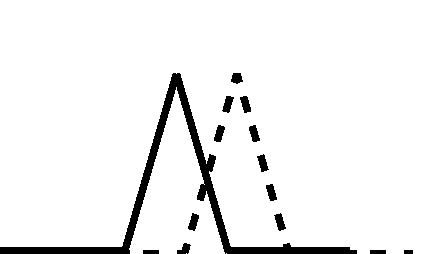
\includegraphics[width=\textwidth]{./figures/invariants/hposition}
 		\caption{Temporal Position}
 	\end{subfigure}
 	~
 	\begin{subfigure}{.45\columnwidth}
 		\includegraphics[width=\textwidth]{./figures/invariants/vposition}
 		\caption{Vertical Position}
 	\end{subfigure}
 	~
 	\begin{subfigure}{.45\columnwidth}
 		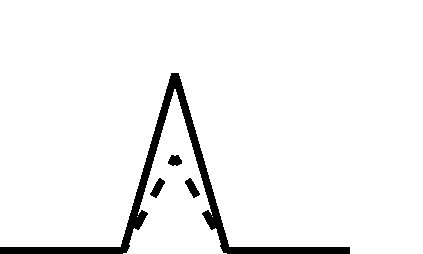
\includegraphics[width=\textwidth]{./figures/invariants/amplitude}
 		\caption{Amplitude}
 	\end{subfigure}
 	~
 	\begin{subfigure}{.45\columnwidth}
 		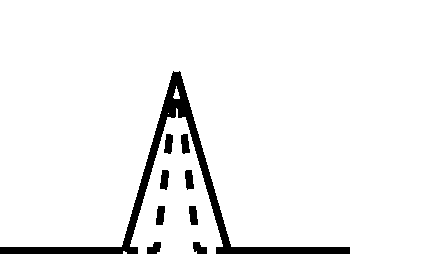
\includegraphics[width=\textwidth]{./figures/invariants/size}
 		\caption{Query Size}
 	\end{subfigure}
 	
 	\begin{subfigure}{.45\columnwidth}
 		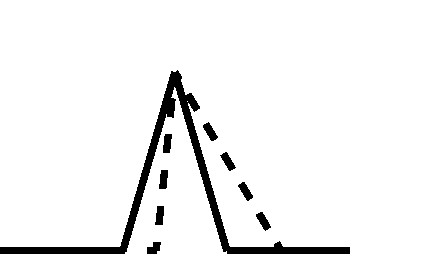
\includegraphics[width=\textwidth]{./figures/invariants/warp}
 		\caption{Time Warp}
 	\end{subfigure}
 	~
 	\begin{subfigure}{.45\columnwidth}
 		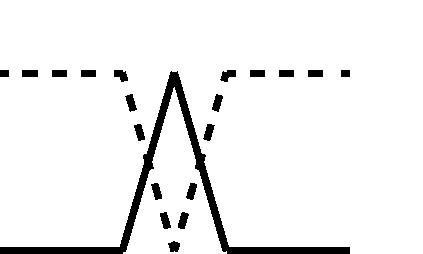
\includegraphics[width=\textwidth]{./figures/invariants/sign}
 		\caption{Sign}
 	\end{subfigure}
 	~
 	\begin{subfigure}{.45\columnwidth}
 		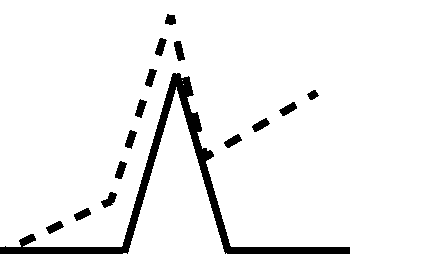
\includegraphics[width=\textwidth]{./figures/invariants/trend}
 		\caption{Trend}
 	\end{subfigure}
 	~
 	\begin{subfigure}{.45\columnwidth}
 		\includegraphics[width=\textwidth]{./figures/invariants/noise}
 		\caption{Noise}
 	\end{subfigure}
 	\caption{A catalog of invariants (or tolerances) for time series matching. For each invariant, assuming a ``spike'' shaped query (the black line), the signal represented by the dotted line would count as a valid match. The analyst's intended meaning of a query might have several implicit or explicit invariants. The analyst might have a different list of what features are or are not relevant during an analysis session. In order to support the analyst, visual query systems ought to flexibly and dynamically support the inclusion or exclusion of these invariants.  }
 	\label{fig:invarlist}
 \end{figure*}	
}

\newcommand{\expFig}{
	\begin{figure*}
		\centering
		\begin{subfigure}[t]{.8\textwidth}
			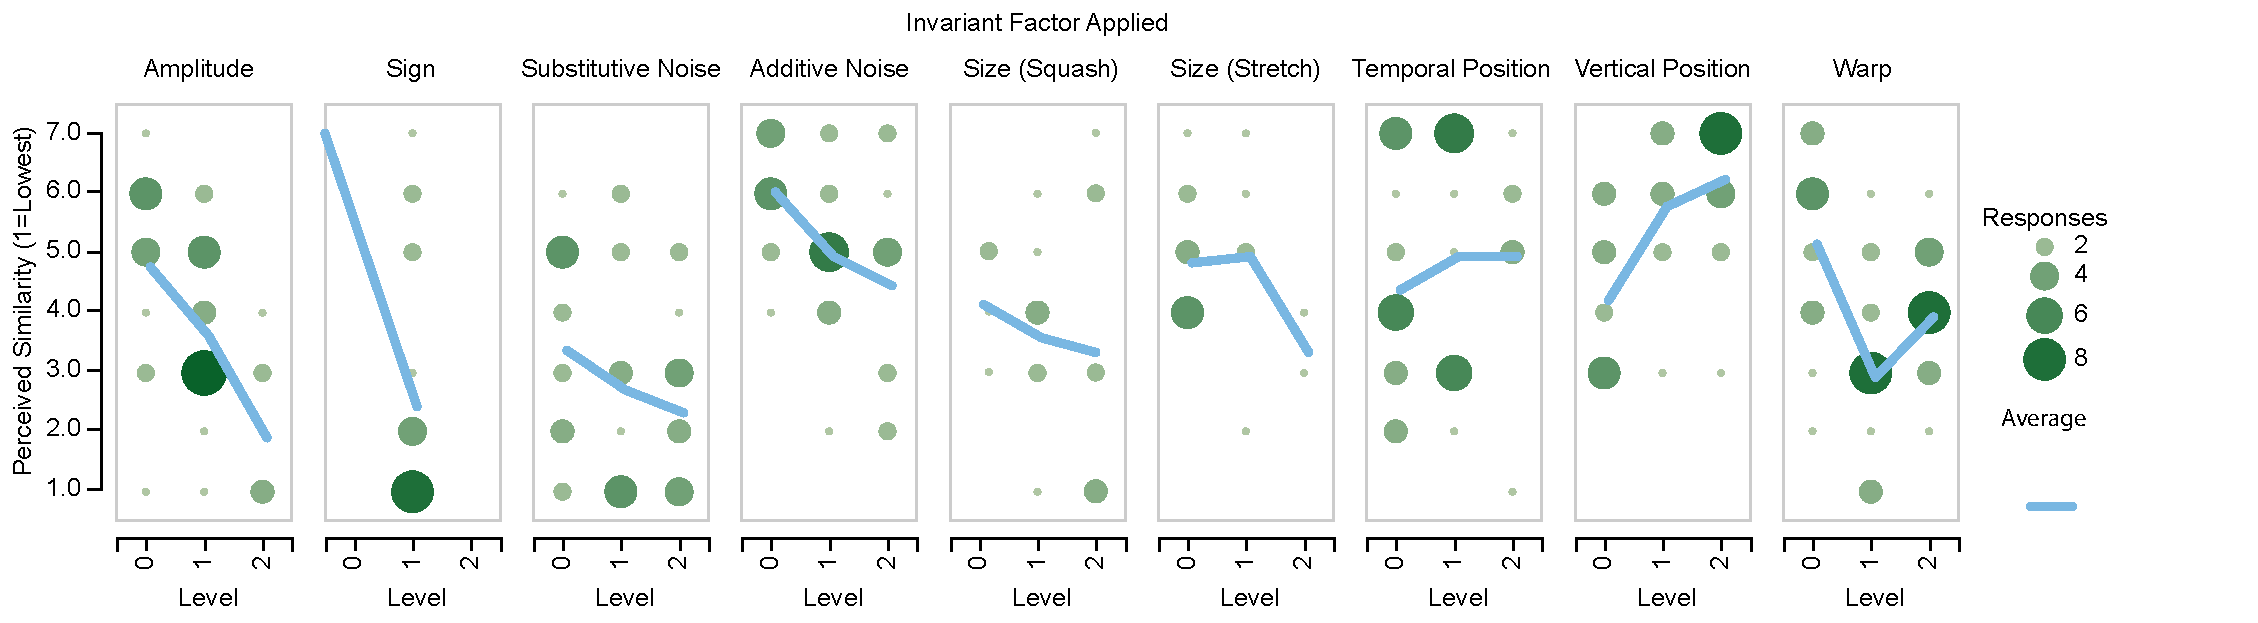
\includegraphics[width=\textwidth]{./figures/exp1-people}
			\caption{Human perceived similarity of area graphs of time series data.}
			\label{fig:exp1people}
		\end{subfigure}
		~
		\begin{subfigure}[t]{.8\textwidth}
			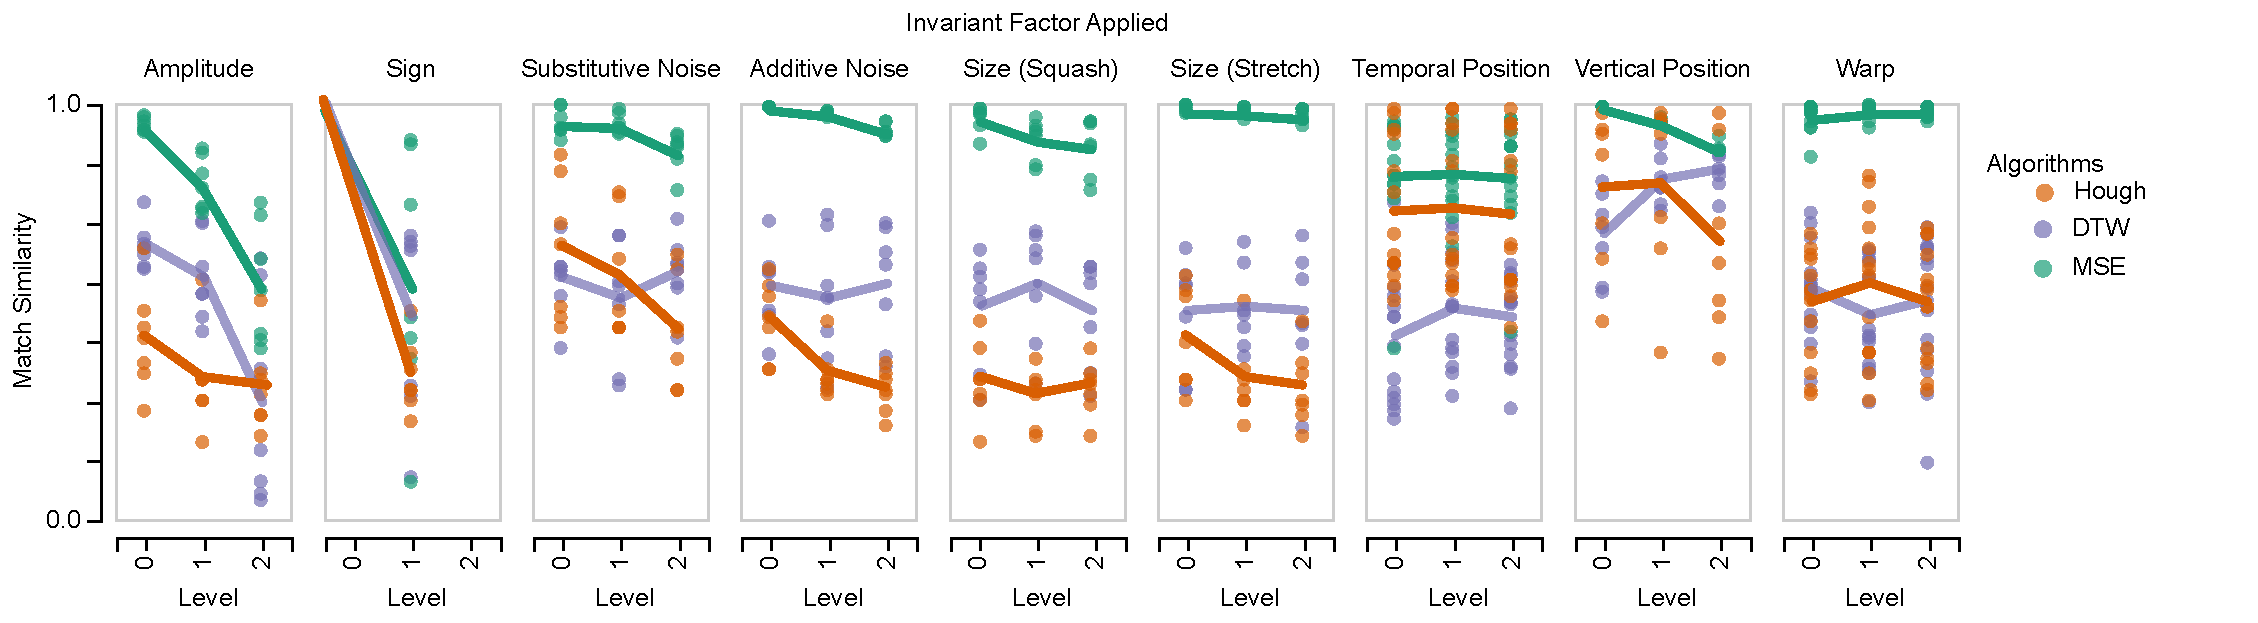
\includegraphics[width=\textwidth]{./figures/exp1-algorithms}
			\caption{Algorithmically calculated similarity. Distances normalized to be in the range $[0,1]$ for each algorithm. }
			\label{fig:exp1algorithms}
		\end{subfigure}
		\caption{Results from our evaluation. Participants were given a target time series, and then had to judge the similarity of the target to a potential match, to which an invariant had been applied. Heterogeneity of human responses show that not all changes to time series result in perceived difference across all viewers. Values are not comparable across conditions, however, slopes are significant: a negative slope represents a sensitivity (similarity falls as the factor increases), while a horizontal line suggests an invariance. This same dataset was then applied to the matching algorithms we present in this paper. Algorithms had varying slopes across the invariants, showing different initial affordances. For instance, additive noise has a significant negative effect on perceived match strength (negative slope). However, only Hough Voting and MSE matching algorithms share a significant negative slope in their match quality as noise is added. Hough Voting and MSE therefore match human judgments of similarity with respect to noise, whereas DTW is invariant to this factor. These data show that algorithmic approaches must be flexible enough to capture the varied mental models of viewers. }
		\label{fig:exp1}
	\end{figure*}
}

\newcommand{\budgetFig}{
	
\begin{figure}
	\centering
	\includegraphics[width=0.7\columnwidth]{./figures/casestudies/budget}
	\caption{A linear query using DTW on the government budget dataset. While some matches have downward slopes, most of the hits have noisy downward trends. We can use these matches to make claims about the presence or absence of patterns in the entire dataset: in this case, agencies tend to lose funding abruptly or noisily, not steadily.}
	\label{fig:budget}
\end{figure}	
}

\newcommand{\eeboFig}{
	
\begin{figure}[h!]
	\centering
	\includegraphics[width=.75\columnwidth]{./figures/casestudies/eebo2.pdf}
	\caption{The top 1000 n-grams from a corpus of 25,000 books printed from 1475-1700 \cite{tcpeebo}. Changes in orthography and print culture over time can create non-standard spellings. In this query, the user has found a decreasing pattern that might indicate a systematic orthographic shift (adding an extraneous `e' to words).}
	\label{fig:eebo}
\end{figure}
}

\newcommand{\stocksFig}{
	
\begin{figure}
	\centering
	\includegraphics[width=.8\columnwidth]{./figures/casestudies/crash.pdf}
	\caption{Our prototype on a dataset of the daily average price of 524 publicly listed stocks over a one year period from 2009 to 2010. The analyst noticed a characteristic dip at roughly the middle of the timespan that seemed to be common. They selected a series with this pattern, and erased all the irrelevant regions, leaving those areas free to vary. By sorting the results in order of match strength, the analyst is able to look past the top few results and see how common this pattern is in the entire dataset. By juxtaposing the top results on the same chart, the analyst can look for patterns of mutual correlation.}
	\label{fig:stocks}
\end{figure}
}

\newcommand{\houghFig}{

\begin{figure}
	\centering
	\begin{subfigure}[t]{.7\columnwidth}
		\includegraphics[width=\textwidth]{./figures/msesquare}
		\caption{A box-shaped query using MSE.}
		\label{fig:msesquare}
	\end{subfigure}
	
	\begin{subfigure}[t]{.7\columnwidth}
		\includegraphics[width=\textwidth]{./figures/houghsquare}
		\caption{A box-shaped query using the Hough Transform.}
		\label{fig:houghsquare}
	\end{subfigure}
	\caption{A box-shaped query on a dataset of the annual budget of 930 U.S. government agencies. MSE will match particular values, finding regions where the budget was, on average, close to the drawn value. Figure \ref{fig:msesquare} shows the results of such a query. Hough voting locates matches that are close in shape to the query, no matter where they occur. Figure \ref{fig:houghsquare} shows these matches, periods of stable budgets.}
	\label{fig:hough}
\end{figure}	
}

\newcommand{\dtwFig}{

\begin{figure}
	\centering
	\begin{subfigure}[t]{.45\columnwidth}
		\includegraphics[width=\textwidth]{./figures/mseyear}
		\caption{A query by example using MSE.}
		\label{fig:mseyear}
	\end{subfigure}
	~
	\begin{subfigure}[t]{.45\columnwidth}
		\includegraphics[width=\textwidth]{./figures/dtwyear}
		\caption{A query by example using DTW.}
		\label{fig:dtwyear}
	\end{subfigure}
	\caption{A query-by-example on the top 1000 words in Google n-grams dataset, based on similarity to the word ``1953.'' Initial scholarship has shown that the words for years have a characteristic spike in popularity as they grow nearer, and then a die-off \protect\cite{michel2011quantitative}. The duration of this die-off is of variable length, and appears to be getting shorter and shorter over time (e.g. the die off for ``1953'' was longer than for ``2003''). This change in event timing is distinct enough that the euclidean distance between year words may be quite different. Figure \protect\ref{fig:mseyear} shows the results from the Mean Squared Error (MSE) metric; there are many potentially irrelevant matches. Figure \protect\ref{fig:dtwyear}, by contrast, uses dynamic time warping to align the series. All of top results are year words, allowing comparison across the dataset.}
	\label{fig:dtw}
\end{figure}	
}

\newcommand{\overviewFig}{

\teaser{
	\centering
	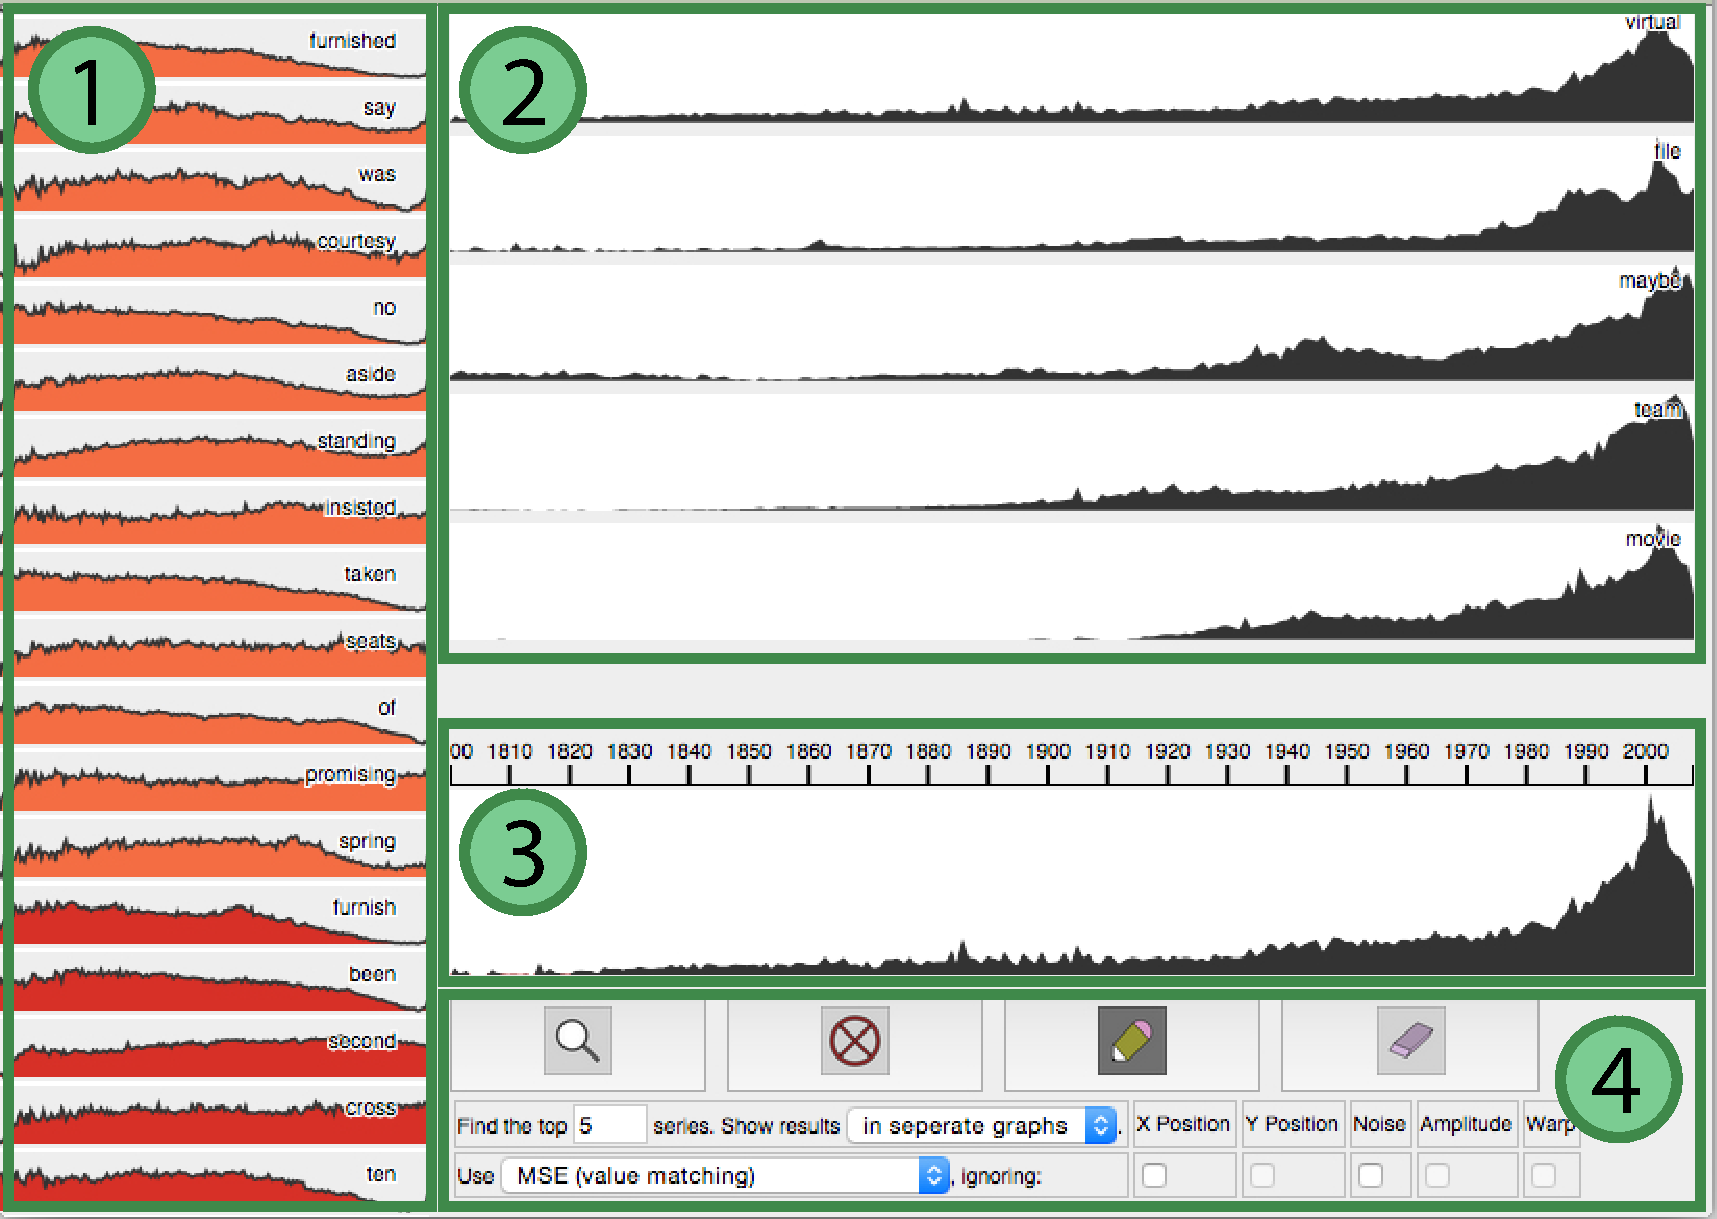
\includegraphics[width=.62\textwidth]{./figures/screenshot2}
	\caption{An overview of the elements of our sketch-based visual query prototype, on the Google N-Grams dataset. Here the analyst wanted to know ``what words have patterns of usage that are most dissimilar to the word `virtual?''' ``Virtual'' is used as a query by example, and the analyst jumps to the bottom of the list of results to find a group of five strong ``anti-matches,'' indicated by their bright red color (including words like ``furnish'' and ``cross''). The components of the system are:
		\\
		\textbf{1}: The scrollable \nameref{sec:smallmultiples} of the entire dataset. Each small multiple is colored according to relative match strength. Here, the analyst has jumped to the bottom of the scroll bar to examine ``anti-matches.''
		\\
		\textbf{2}: The \nameref{sec:results}, showing the top $k$ results for a query. The analyst selects how many results they wish to consider, and whether these results are superimposed in the same plot, or drawn as separate line graphs.
		\\
		\textbf{3}: The \nameref{sec:drawing}. The analyst can sketch their own queries here, or, as in this example, use an existing time series as a base for sketching.
		\\
		\textbf{4}: The \nameref{sec:query} interface and general UI. The large top buttons allow users to execute queries, clear the canvas, draw on the canvas, or erase portions of the canvas, respectively. The lower levels control how results are displayed and what invariants are active.}
	\label{fig:overview}
	}
}

\newcommand{\overviewFigStar}{
	
	\begin{figure*}
		\centering
		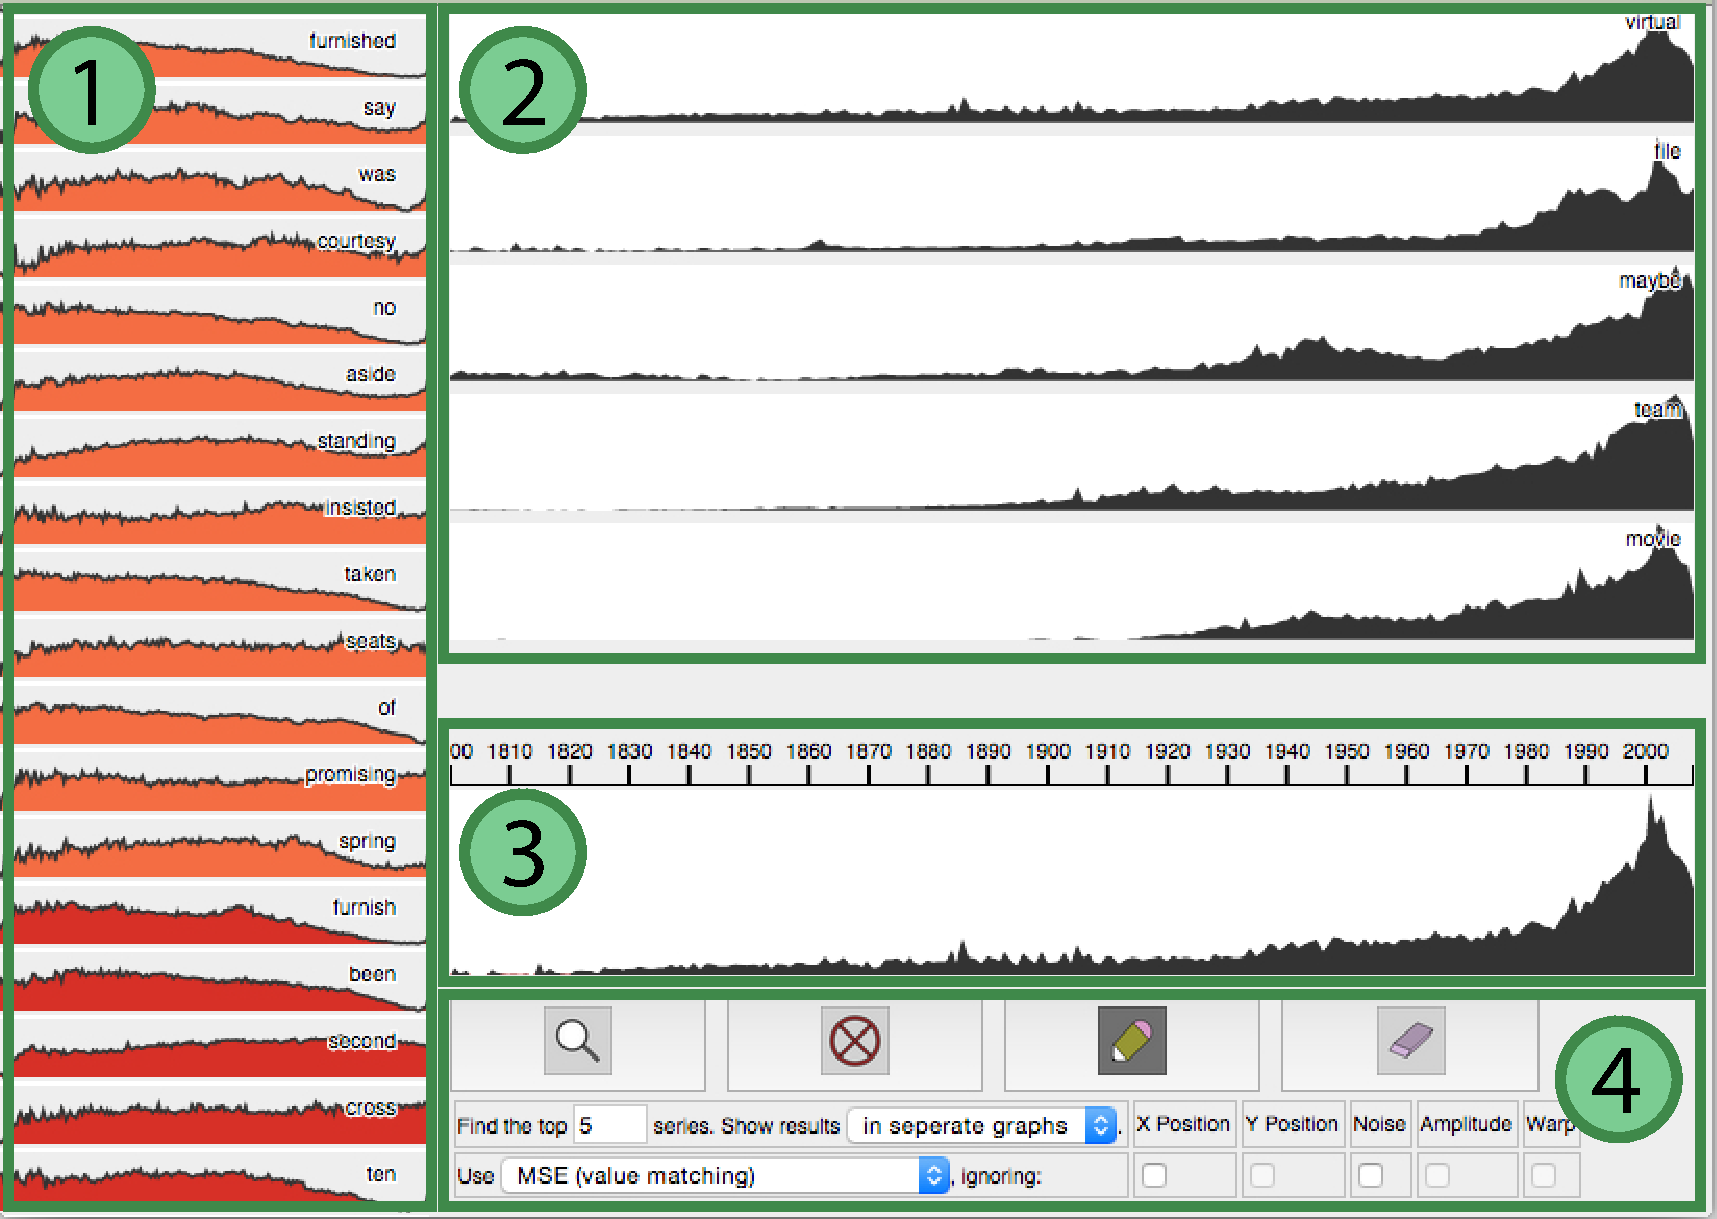
\includegraphics[width=.62\textwidth]{./figures/screenshot2}
		\caption{An overview of the elements of our sketch-based visual query prototype, on the Google N-Grams dataset. Here the analyst wanted to know ``what words have patterns of usage that are most dissimilar to the word `virtual?''' ``Virtual'' is used as a query by example, and the analyst jumps to the bottom of the list of results to find a group of five strong ``anti-matches,'' indicated by their bright red color (including words like ``furnish'' and ``cross''). The components of the system are:
			\\
			\textbf{1}: The scrollable \nameref{sec:smallmultiples} of the entire dataset. Each small multiple is colored according to relative match strength. Here, the analyst has jumped to the bottom of the scroll bar to examine ``anti-matches.''
			\\
			\textbf{2}: The \nameref{sec:results}, showing the top $k$ results for a query. The analyst selects how many results they wish to consider, and whether these results are superimposed in the same plot, or drawn as separate line graphs.
			\\
			\textbf{3}: The \nameref{sec:drawing}. The analyst can sketch their own queries here, or, as in this example, use an existing time series as a base for sketching.
			\\
			\textbf{4}: The \nameref{sec:query} interface and general UI. The large top buttons allow users to execute queries, clear the canvas, draw on the canvas, or erase portions of the canvas, respectively. The lower levels control how results are displayed and what invariants are active.}
		\label{fig:overview}
	\end{figure*}
}

\newcommand{\invariancesFig}{

\begin{figure*}
	\centering
	\begin{subfigure}[t]{.25\textwidth}
		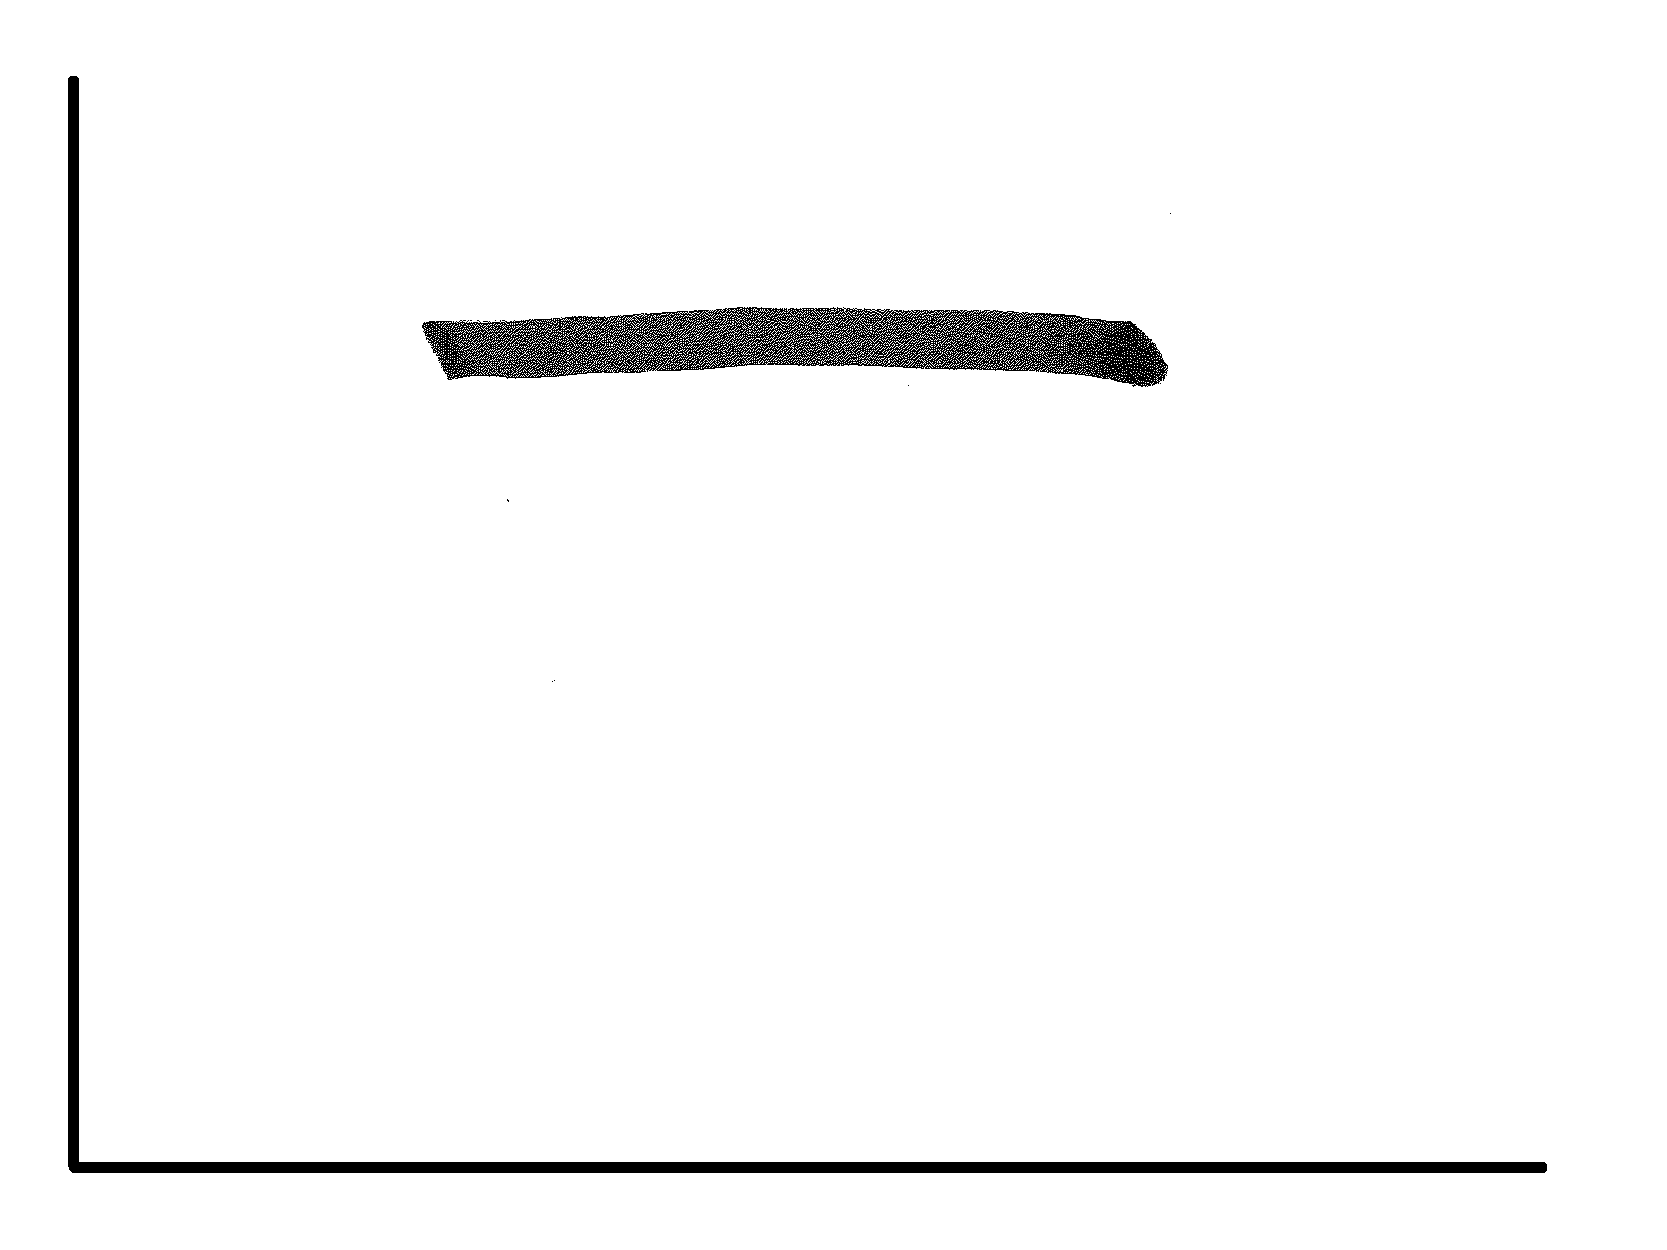
\includegraphics[width=\textwidth]{./figures/sketch2}
		\caption{An input sketch. What counts as a match to this input?}
		\label{fig:sketch}
	\end{subfigure}
	~
	\begin{subfigure}[t]{.25\textwidth}
		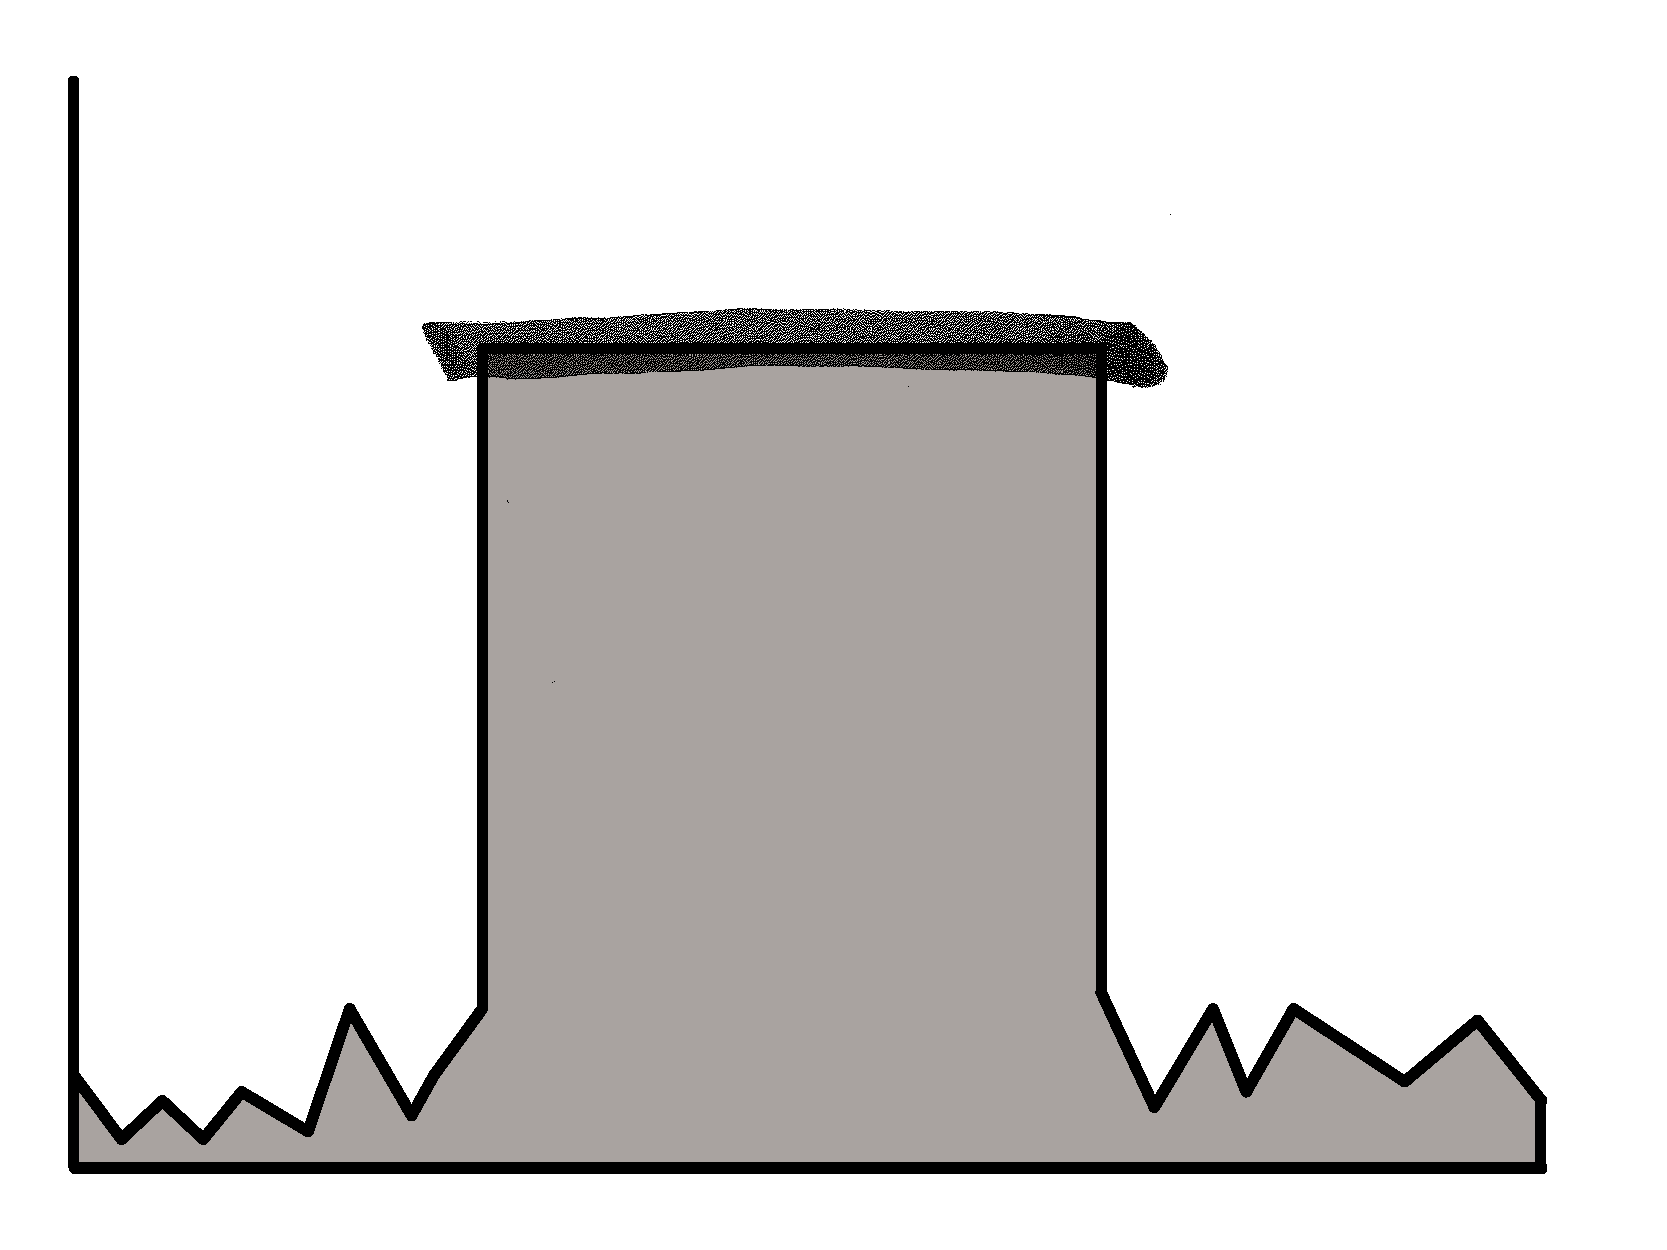
\includegraphics[width=\textwidth]{./figures/exact}
		\caption{A match where, if there is no sketch information, the query is interpreted as being zero.}
		\label{fig:zeroval}
	\end{subfigure}
	~
	\begin{subfigure}[t]{.25\textwidth}
		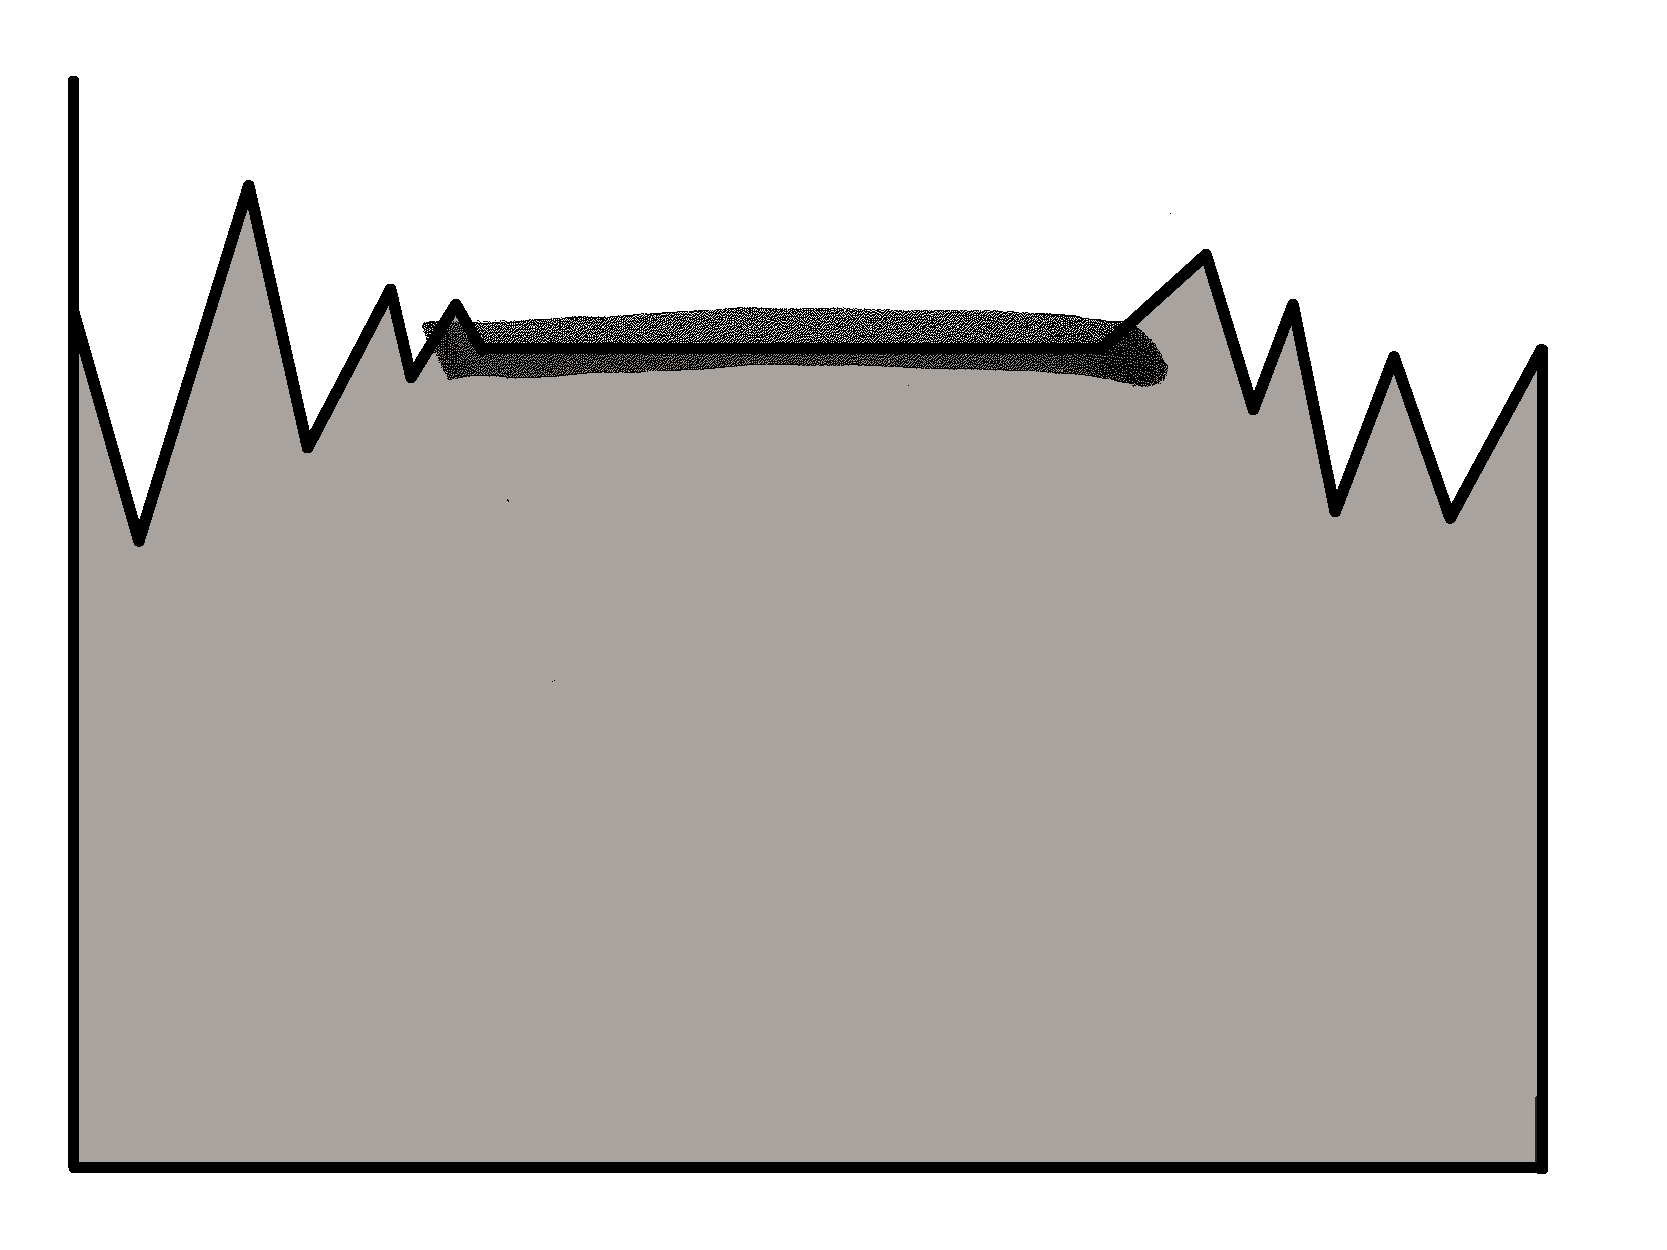
\includegraphics[width=\textwidth]{./figures/dontcare}
		\caption{A match where, if there is no sketch information, arbitrary values will match the query. }
		\label{fig:dontcare}
	\end{subfigure}
	
	
	\begin{subfigure}[t]{.25\textwidth}
		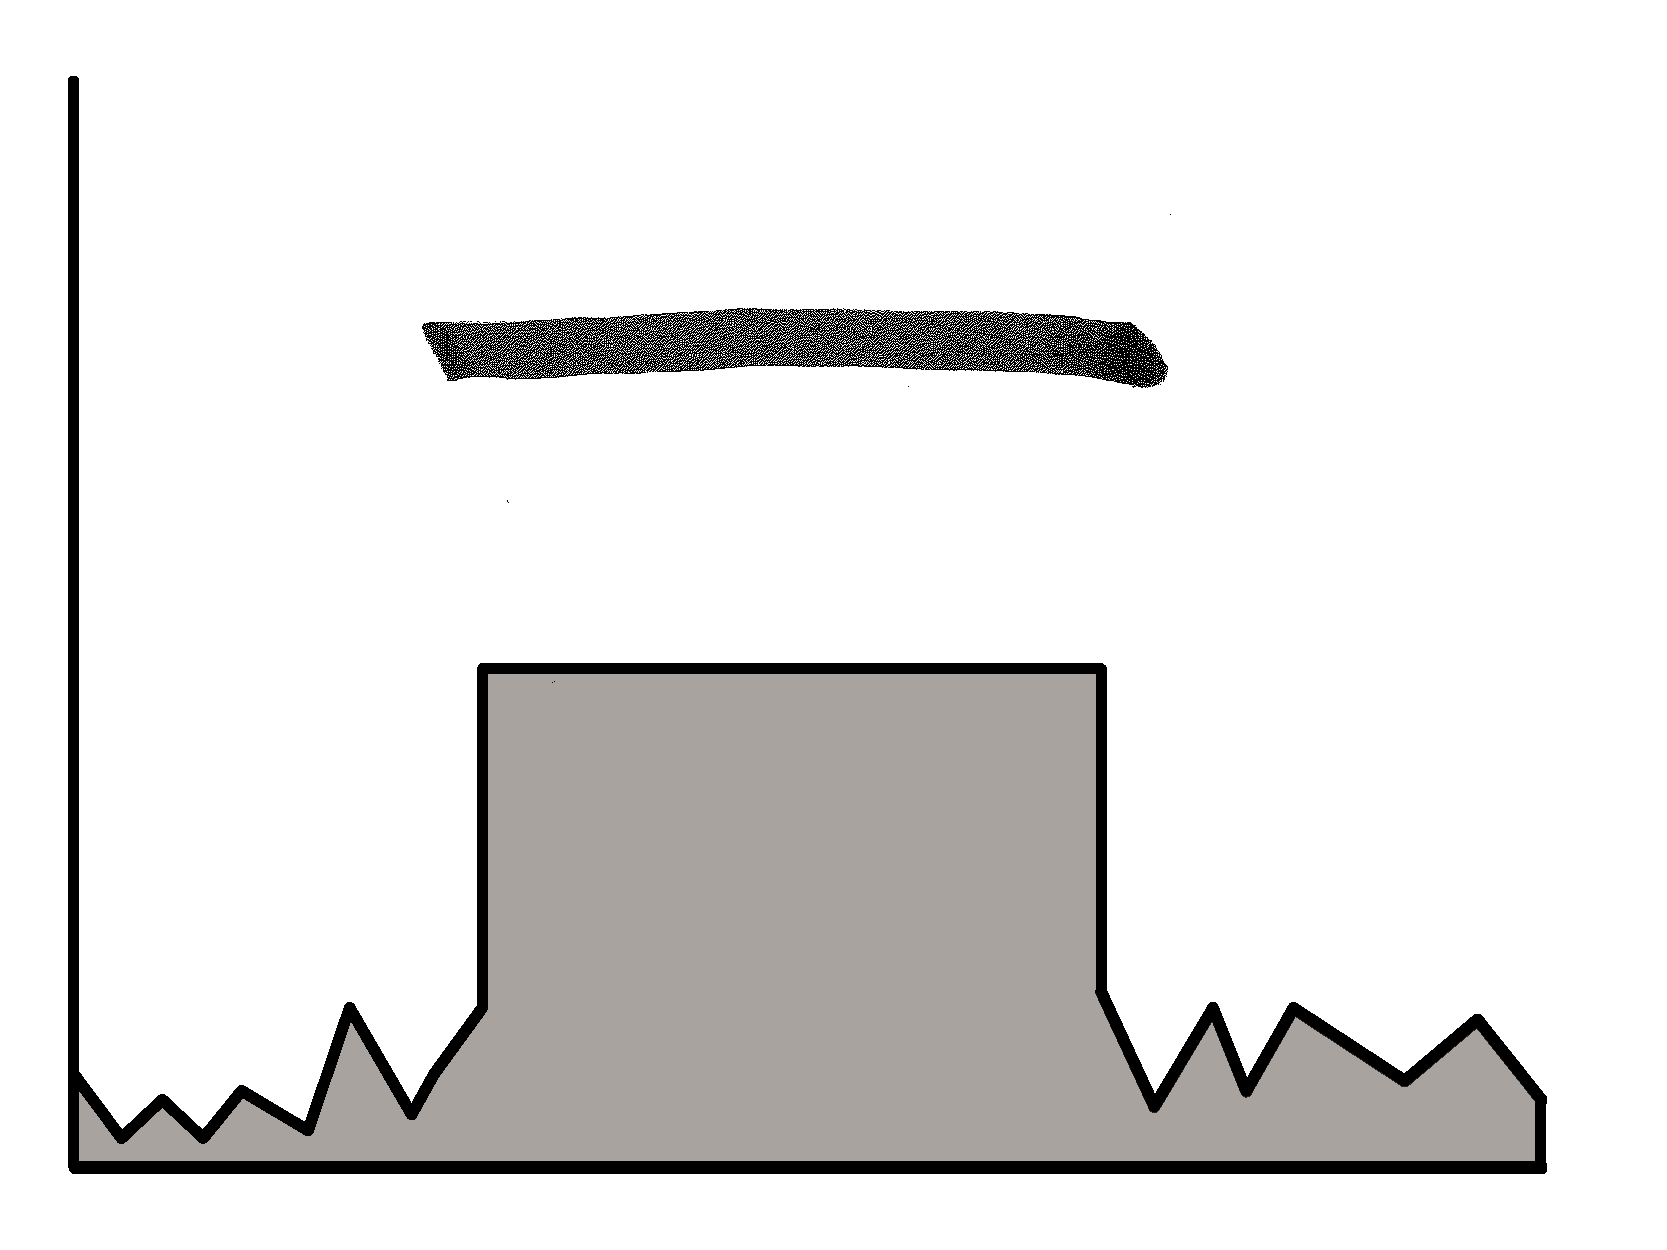
\includegraphics[width=\textwidth]{./figures/amplitude}
		\caption{A match in visual \emph{shape}, but not in \emph{value}.}
		\label{fig:pattern}
	\end{subfigure}
	~
	\begin{subfigure}[t]{.25\textwidth}
		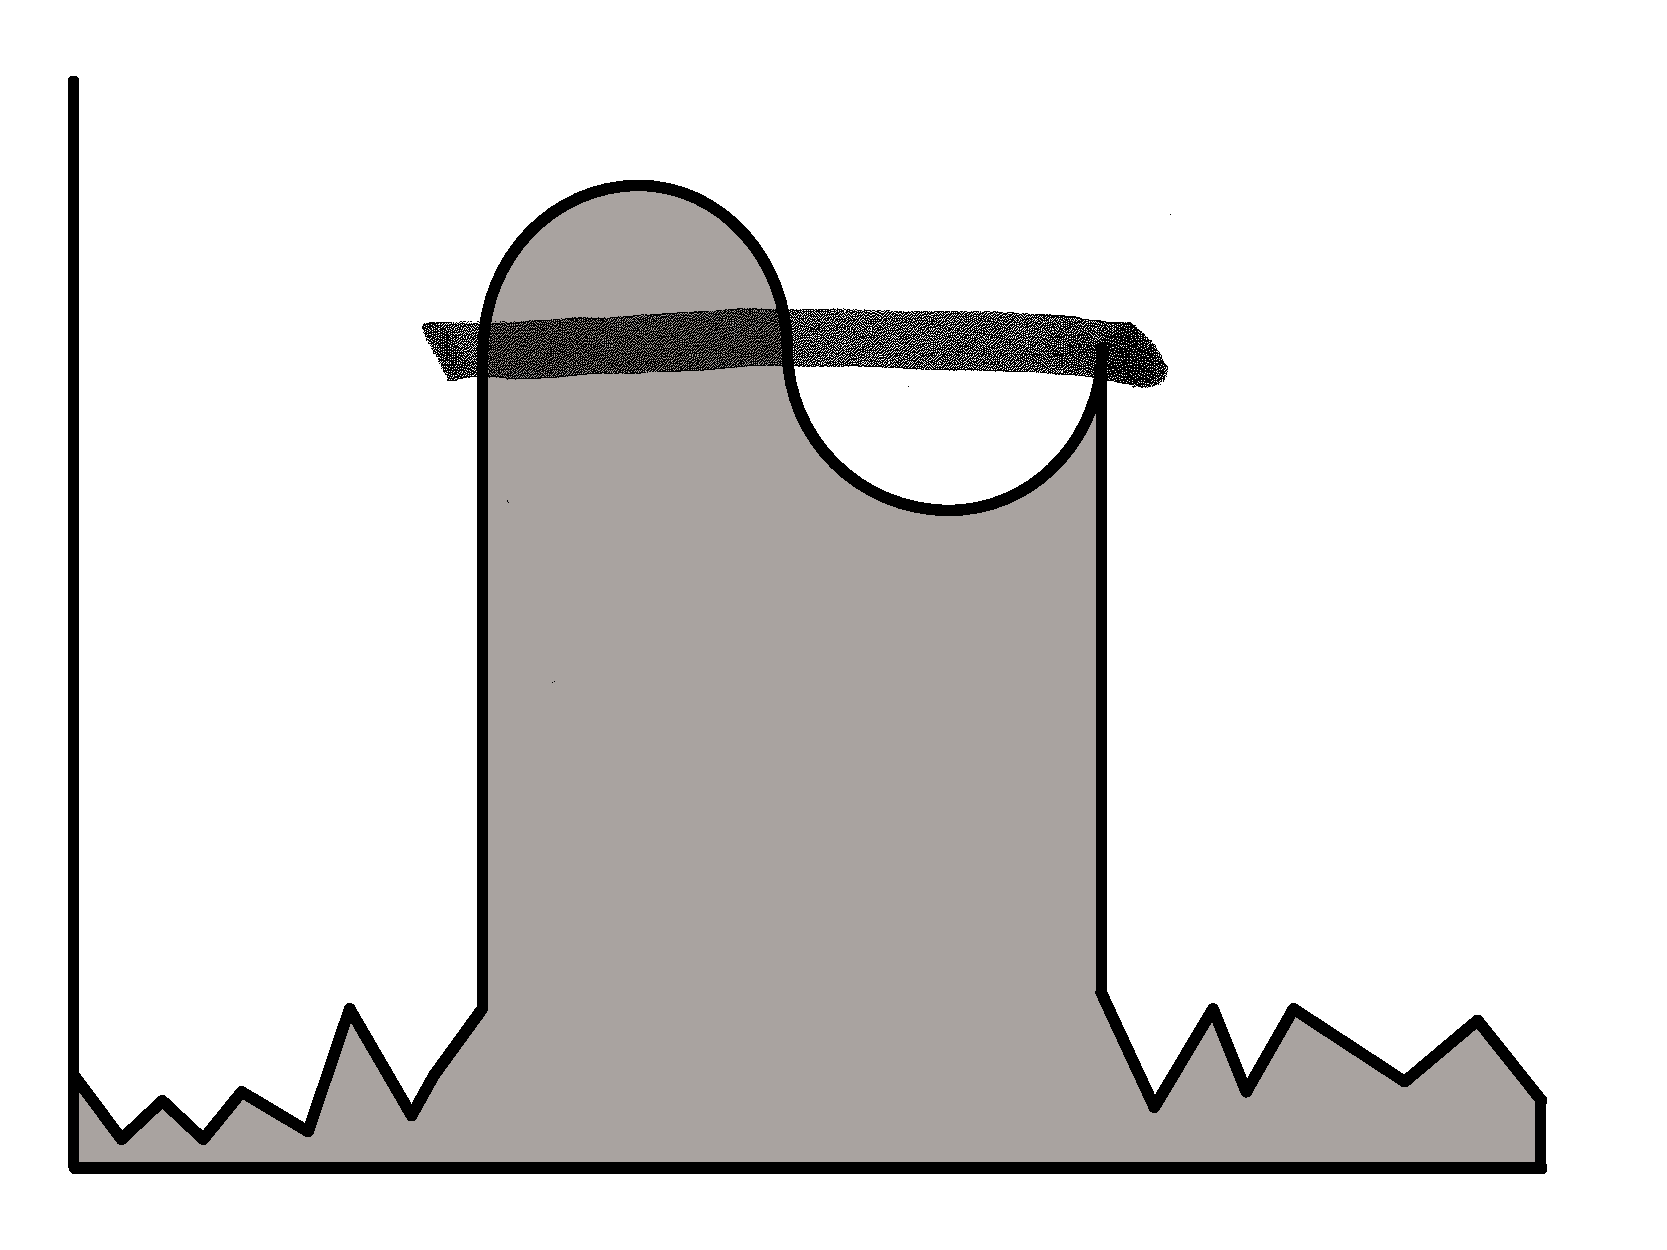
\includegraphics[width=\textwidth]{./figures/average}
		\caption{A match in average \emph{value} but not \emph{shape}.}
		\label{fig:value}
	\end{subfigure}
	~
	\begin{subfigure}[t]{.25\textwidth}
		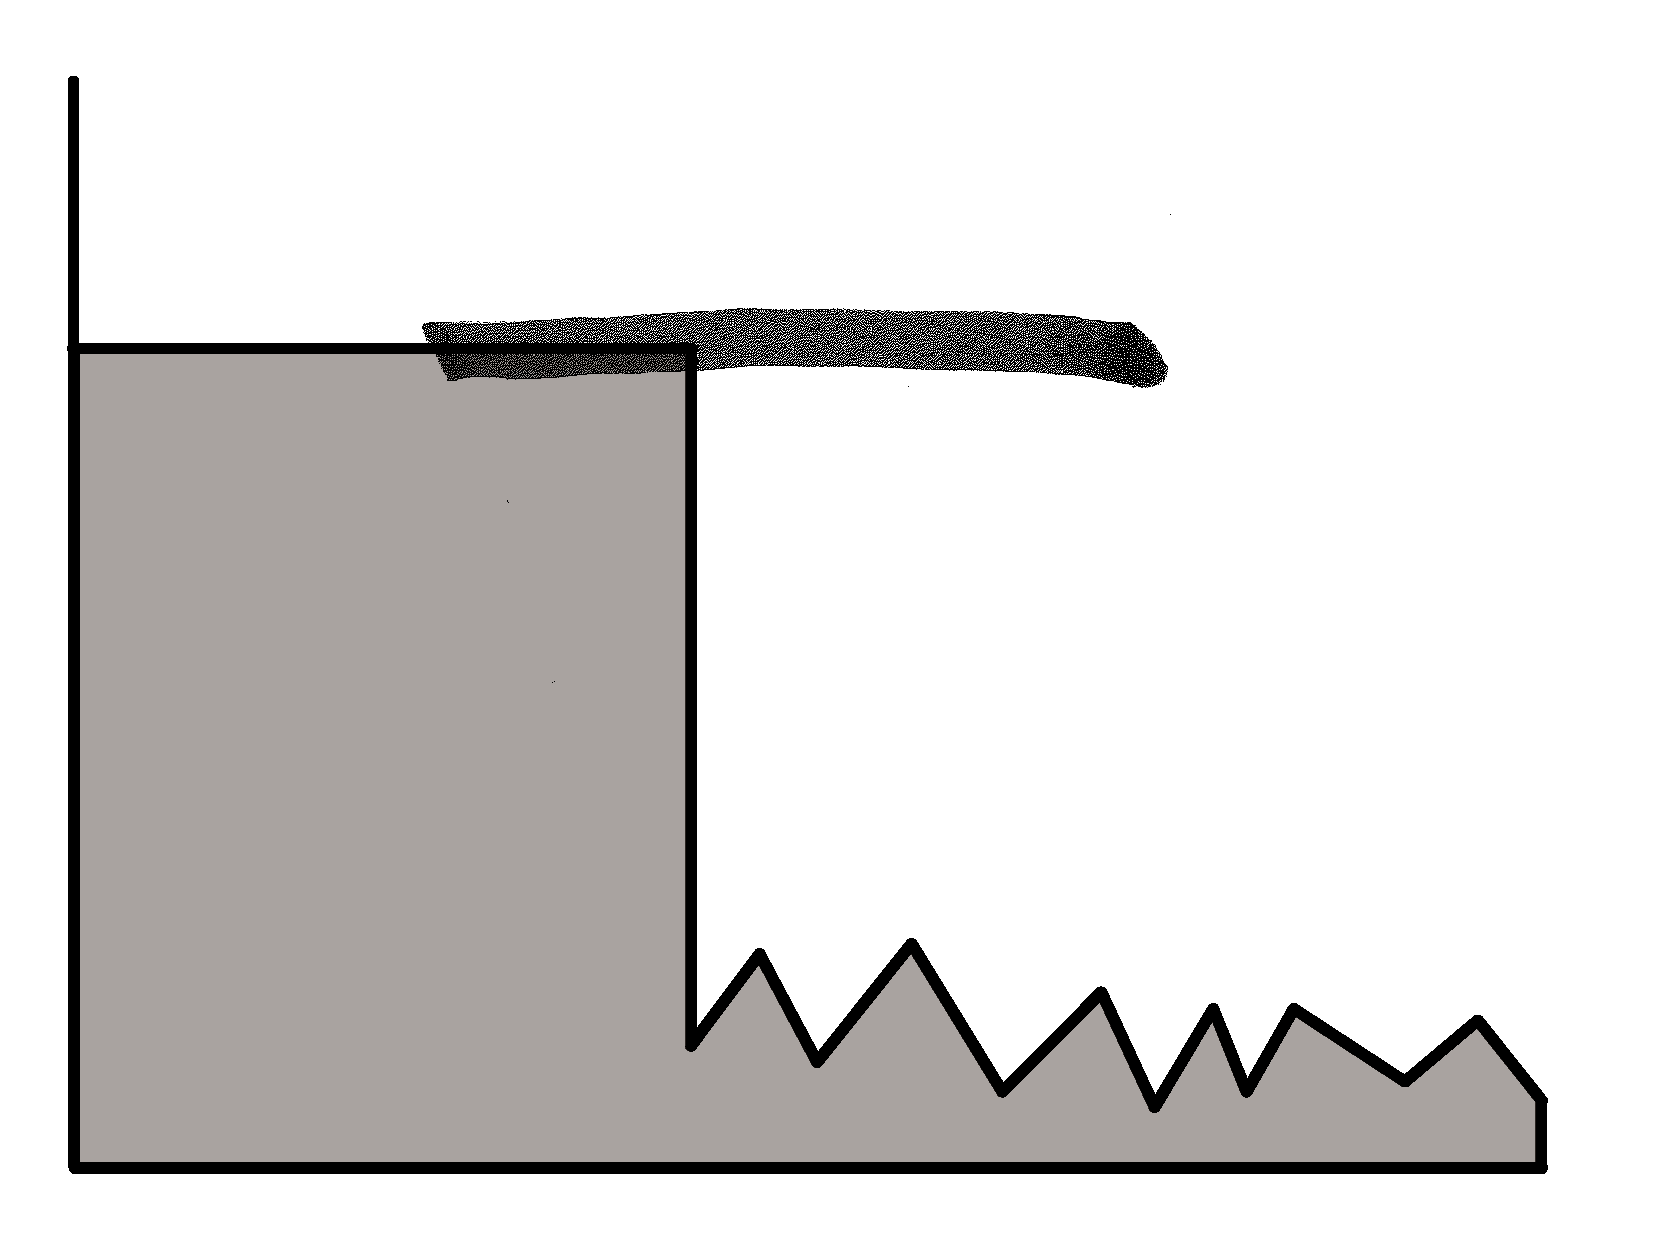
\includegraphics[width=\textwidth]{./figures/temporal}
		\caption{A match that occurs in a different temporal location than in the sketch.}
	\end{subfigure}
	\caption{An example of the ambiguity of sketches as queries. A single sketch can produce many potential matches based on the semantic interpretation of the sketch. Some of these differences can be characterized by one or more invariants (does the analyst care about amplitude, temporal shifts, or noise?), but other differences are fundamental (how should missing values be treated? Should matches be based on the \emph{pattern} of the sketch, or the explicit \emph{values} in the sketch?). These decisions may change over the course of an analysis session. Therefore, visual query systems must provide the option for the analyst to adjust invariants dynamically.}
	\label{fig:invariances}
\end{figure*}
}

\newcommand{\targetFig}{
	
	\begin{figure}
		\centering
		\begin{subfigure}[t]{.45\columnwidth}
			\includegraphics[width=\textwidth]{./figures/targets/0}
			\caption{Upwards Line}
		\end{subfigure}
		~
		\begin{subfigure}[t]{.45\columnwidth}
			\includegraphics[width=\textwidth]{./figures/targets/0_a}
			\caption{Amplitude}
		\end{subfigure}
	
		\begin{subfigure}[t]{.45\columnwidth}
			\includegraphics[width=\textwidth]{./figures/targets/1}
			\caption{Downwards Line}
		\end{subfigure}
		~
		\begin{subfigure}[t]{.45\columnwidth}
			\includegraphics[width=\textwidth]{./figures/targets/1_i}
			\caption{Sign}
		\end{subfigure}	
		
		\begin{subfigure}[t]{.45\columnwidth}
			\includegraphics[width=\textwidth]{./figures/targets/2}
			\caption{Sine Wave}
		\end{subfigure}
		~
		\begin{subfigure}[t]{.45\columnwidth}
			\includegraphics[width=\textwidth]{./figures/targets/2_n}
			\caption{Noise}
		    \label{fig:noisetarget}
		\end{subfigure}	

		\begin{subfigure}[t]{.45\columnwidth}
			\includegraphics[width=\textwidth]{./figures/targets/3}
			\caption{Tent}
		\end{subfigure}
		~
		\begin{subfigure}[t]{.45\columnwidth}
			\includegraphics[width=\textwidth]{./figures/targets/3_s}
			\caption{Query Size}
		\end{subfigure}	
			
		\begin{subfigure}[t]{.45\columnwidth}
			\includegraphics[width=\textwidth]{./figures/targets/4}
			\caption{Perlin Noise v.1}
		\end{subfigure}
		~
		\begin{subfigure}[t]{.45\columnwidth}
			\includegraphics[width=\textwidth]{./figures/targets/4_t}
			\caption{Temporal Position}
		\end{subfigure}	
		
		\begin{subfigure}[t]{.45\columnwidth}
			\includegraphics[width=\textwidth]{./figures/targets/5}
			\caption{Perlin Noise v.2}
		\end{subfigure}
		~
		\begin{subfigure}[t]{.45\columnwidth}
			\includegraphics[width=\textwidth]{./figures/targets/5_v}
			\caption{Vertical Position}
		\end{subfigure}	
		
		\begin{subfigure}[t]{.45\columnwidth}
			\includegraphics[width=\textwidth]{./figures/targets/6}
			\caption{Parabola}
		\end{subfigure}
		~
		\begin{subfigure}[t]{.45\columnwidth}
			\includegraphics[width=\textwidth]{./figures/targets/6_w}
			\caption{Time Warp}
		\end{subfigure}			
									
		\caption{A full list of the targets from our evaluation, and examples of invariant factors. We generate a pseudo match by applying a factor, and then adding noise to the rest of the series.Two different targets representing pseudo-random noise were used. Additionally, we considered two different characteristics of noise. Substitutive (Fig. \ref{fig:noisetarget}), and additive (not shown).}
		\label{fig:targets}
	\end{figure}
}